
\begin{figure}[h]
  \centering
  \begin{tabular}{  c p{0.7cm} c }
    \centering
    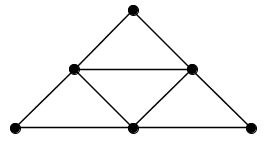
\includegraphics[width=4cm]{img/s3.png} & &
    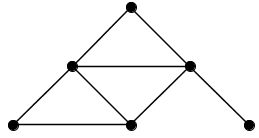
\includegraphics[width=4cm]{img/s3-1.png}
    \\
    \footnotesize \centering 
    (a)  \footnotesize Grafo $S_3$. &&  \footnotesize (b) Grafo $S_{3'}$. \\
    
    %---------------------
      \centering 
      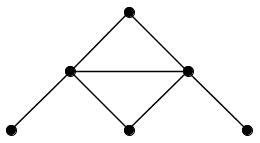
\includegraphics[width=4cm]{img/s3-2.png} & &
    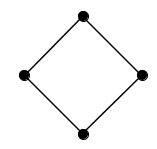
\includegraphics[width=3cm]{img/c4.png}
    \\
    \footnotesize \centering 
    (c)  \footnotesize Grafo $S_{3''}$. && \footnotesize (b) Grafo $C_{4}$.\\
  \end{tabular}

 \caption{Grafos do enunciado do  Teorema~\ref{lem:chordalDiamondFree}.}
 \label{fig:proibidos}
\end{figure} 
